%*************************************************
\section{DBaaS information leakage management}
\label{LeakagePreventionSection}
%*************************************************
In databases, there are often unknown correlations among the heterogeneous data types beyond defined dependencies such as primary or foreign keys relationship between attributes. From the data security point of view, since the analysis of the hidden correlations reveals sensitive information, it is desired to minimize the correlation leakage especially in an untrusted outsourced server. However, it is a demanding goal because there is no well-known measure to quantify the attributes correlations.\\

We propose two quantifying methods for attributes correlation analysis: First, the \emph{explicit correlation} can be formed due to the exact match relation between the attributes. The advised quantification function operates based on tracking and matching the occurrence of exact key and value matching in different databases, and associates a non-negative real value for any correlation. The assigned number represents the level of the leaked information from pooling any given pair of documents. We adopt the recall and precision concepts to quantify exact match correlation leakage.\\ 


Statistical properties of attributes (even heterogeneous data types) within documents generates an unintended \emph{implicit correlation} that leaks private information. The detection of implicit information dependences are very complicated, and requires deep statistical analysis of attributes' properties. For instance, often the correlations between energy consumption and area of a building or the number of occupants leaks valuable information. As a second clarifying example, there is a correlation between illness and the corresponding medication that is prescribed for an individual. The quantification of correlation as a result of statistical property is addressed in our second approach.\\


Conceptually, the data warehouse used for DBaaS warehouse can be considered as a new higher layer coarse-grained storage that operates in multiple enterprise level. DBaaS hosts vast number of databases belong to enterprises, and each dataset contains a set of documents. In this work, the DBaaS repository is represented by $W_{DBaaS}$ which is a set of databases, and information leakage caused by the attribute correlation is formulated as follows:

\[
W_{DBaaS}=\Big \langle D_1,\dots,D_n \Big \rangle
\]
Each database $D_\imath ~, ~~ 1\leqslant \imath \leqslant n$ consists of a set of arbitrary number  $m$ of documents.
\[
D_\imath=\big\{ d_1,\dots,d_m\big\}\\
\] 
Eventually, documents are defined as a set of attributes which are appointed as the fine-grained level of cloud data warehouse. Each document $d_\jmath~,~~1\leqslant \jmath \leqslant m$ are comprised of an arbitrary number $l$ attributes which are basically built up with a key-value pair $\langle key, value\rangle$. 
\[
d_\jmath=\big\{ A_1,\dots, A_l\big\} 
\]
The major types of attribute correlation leakage are discussed in the following subsections and the corresponding sub-optimal solutions to minimize the leakage are proposed.

%*************************************************
\subsection{Attribute correlation leakage prevention with disinformation}
\label{AttributeCorrelationSubsection}
%*************************************************
In this section, two types of attribute correlation leading to information leakage are investigated and and leakage management solution involving insertion of disinformation insertion is proposed with their corresponding examples. 

%*************************************************
\subsubsection{Explicit correlation}
\label{ExplicitCorrelationSubsection}
%*************************************************

An attribute correlation between any two collections (databases) is described as a frequent occurrence of the attributes values in the different collections that are stored in the same cloud data warehouse. A correlation function assigns a non-negative real number value as correlation score to a group of datasets. The correlation function, also denoted as $\Psi_{\epsilon}(D_P,D_Q)$, extracts the leakage between two databases $D_p$ and $D_q$, that indicates the amount of leaked information as a result of existing correlations. Equation \ref{eq:attributeCorrelation} formulates correlation function.

\begin{equation}
\label{eq:attributeCorrelation}
\begin{aligned}
\Psi (D_P,\mathcal{D}_Q):
& \forall~d_p \in D_P ~\land~ \forall~ d_q \in D_Q ~~if~~ (\mu(d_p,d_q)==True) \implies \mathcal{L}=d_p~ \Delta ~d_q 
\end{aligned}
\end{equation}
Where $\mathcal{L}$ is the leakage factor and the operator $\Delta$ is defined as $d_p~ \Delta ~d_q =(d_p\setminus d_q)\cup (d_q\setminus d_p)$.\\

The feasibility function $\mu$ determines if a given pair of documents are capable of being merged using attributes classification. In other words, the µ function returns true for a pair of documents that share any number of identifier attributes (one or more). Also, for multiple semi-identifier attributes that can collectively identify an entity in the scope of dataset, the returned value of the feasibility function is true. Equation \ref{eq:muFunction} outlines this function.


\begin{equation}
\label{eq:muFunction}
\begin{aligned}
& \mu(d_p,d_q)= \begin{cases}
&\textbf{True} \\
&iff \quad \exists A_r \in d_p ~ \land ~\exists A_s \in d_q ~ \mid [(A_r.key==A_s.key) \land (A_r.value==A_s.value)]\\
\noalign{\text{such that $A_r, A_s$ are indentifier attributes of $d_p, d_p$}}\\
&\textbf{False} \qquad Otherwise
\end{cases}\\
\end{aligned}
\end{equation}\\
The leakage factor $\mathcal{L}$ represents volume of leaked information from two arbitrary documents $d_p, d_q$ due to the existence of one or more identifier in both documents. Note that these documents can be chosen from one or two different collections. A fundamental requirement to manage the amount of information leakage,  is to introduce measurement metrics. The first metric we developed, is basically the improved version of the metric that was introduced by Whang et al.\cite{whang2010managing}. The well-known \emph{precision} and \emph{recall} concepts were adopted from data retrieval to measure the information leakage. Precision is defined as the ratio of the number of attributes in a document $d$ to the number of attributes in the reference document. In Whang et al method, an equal weight has been assigned to all the attributes, while, we improved this model by varying  the weight of attributes according to their type.

\noindent For accurate quantifying of information leakage, a notion $ \Omega$ is defined as a quantitative metric for representing the value of information stored in a document $d$. This metric is the summation of $0 \leq \omega_\imath \leq 1$ which is associated for any attribute $A_\imath$ in the document, obtained by $\Omega=\sum\limits_{\imath=1}^n \omega_\imath$. The higher magnitude of the corresponding
$\omega_\imath$ value reflects the importance of an attribute $A_\imath=\{key, value\}$. Consequently, for any document $d$ the value of $\Omega$determines the value of all information in the document. The highest possible value  $\omega_\imath = 1$ is assigned to the identifier attributes. The weight value for a group of $m$ semi-identifier attributes that collectively identify an entity, is assigned to be  $\omega_\imath=\frac{1}{m}$. Moreover, a feature attribute receives a very small $\omega_\imath$ value. Equation \ref{eq:weightedRecallPrecison} represents the weight calculation for any given document.\\

\begin{equation}
\label{eq:weightedRecallPrecison}
\begin{aligned}
& \Omega_d=\alpha \times n + \beta \times m + \gamma \times p \qquad
 Such~ that:~ \alpha \gg \beta \gg \gamma \geq 0
\end{aligned}
\end{equation}
Where $n$ is the number of identifier attributes with weight $\alpha$, $m$ is the number of semi-identifier attributes with weight $\beta$, and $p$ is the number of feature attributes with weight $\gamma$.


As a result of dynamic schema employed for data model, in the context of the NoSQL database, the documents related to the same object are allowed to have various number of attributes. However, a full list of attributes is necessary to create a reference document. Therefore, we define a logical operator $\delta$ denoted as \emph{Super Document}, that aggregates all attributes related to an entity in the scope of collection to create the reference document required for precision and recall. 

Apparently, the cloud insider has a wide view scope in terms of accessible data for $\delta$ function. Having comprehensive super document is impractical; however, it can be called for any subset of the selected databases (one or more). To construct a super document of an entity from set of collections, first the super document is initialized with a document that describes the entity ($d_i$). Second, the other documents ($d_j$) are scanned to extract any undetected attributes of the entity, $\mathcal{L}(\delta_{\imath},d_\jmath)$.The Equation \ref{eq:SuperDocument} demonstrates the notion of super document. The construction of a super document from multiple data collections is described in Algorithm \ref{algo:ExractingLeakedInformation} (see Appendix \ref{app:Algorithms}).

\begin{equation}
\label{eq:SuperDocument}
\begin{aligned}
\begin{cases}
&\delta_{\imath}=d_\imath \\
&\forall d_\jmath \in \mathcal{D}, \quad \delta_{\imath}= \delta_{\imath} \cup \mathcal{L}(\delta_{\imath},d_\jmath)
\end{cases}
\end{aligned}
\end{equation}


Measurement of information leakage in the document level with utilization of $\delta$ function (super document) and $\omega_i$ value, for precision and recall metrics is straightforward computation. The process to figure out $\delta$ function among the multiple collections that are hosted by the same cloud DBaaS is outlined in the Algorithm \ref{algo:ExractingLeakedInformation}. If a new attribute is extracted, it will be appended to the super document, then a back track is needed in order to check for new paths which were already closed. The search space raises exponentially according to the number of attributes.

In order to break the correlation between documents, we intentionally insert documents containing false or misleading values for sensitive attributes denoted as \emph{disinformation document} which includes common attributes shared with the original document. As a result of disinformation document insertion, the extraction of new attributes value from correlation will be more expensive for an attacker by factor of the number of disinformation per original document. 


\noindent \textsc{\textbf{Example 1.}} Consider five documents from different databases selected from the DBaaS warehouse, belonging to two individuals. The goal is to extract leaked information using attribute correlation. This case exemplifies Algorithm \ref{algo:ExractingLeakedInformation} presented in Appendix \ref{app:Algorithms} and table \ref{tab:weightTable} shows the list of attributes for this example with hypothetical weight.




\begin{table*}[htp]
\caption{Weights of attributes}
\label{tab:weightTable}
\centering
\begin{tabular}{lcc}
\toprule
\textbf{Attribute} & \textbf{Type} & \textbf{$\omega$}\\
\midrule
Zip      & Semi-identifier  & 0.3 \\ 
Address  & Semi-identifier  & 0.5 \\
Phone    & identifier       & 1.0 \\
Account  & identifier       & 1.0 \\
Name     & Semi-identifier  & 0.6 \\
Age      & Feature          & 0.1 \\
Income   & Feature          & 0.1 \\
SSN      & identifier       & 1.0 \\
Email    & identifier       & 1.0 \\
\bottomrule
\end{tabular}
\end{table*}

\begin{align*}
d_1&=\{ {\bf zip} : 456 ,~{\bf address}:``2512~ Uni.~NY",~ phone:\underline{111}\}\\
d_2&=\{ {\bf ssn} : 123,~ {\bf age} : 33,~ {\bf account}: 222 \}\\
d_3&=\{ {\bf name} : ``Kate~Jones",~ {\bf age} : 30,~ {\bf address}: ``abc",{\bf email}:``kj@a.com" \}\\
d_4&=\{ {\bf name} : ``Mike~Smith", {\bf income} :70k,~ {\bf ssn}:123, ~ {\bf phone}:\underline{111}\}\\
d_5&=\{ {\bf name} : ``Kate~Jones",{\bf email}:``kj@a.com",~ {\bf ssn} : 777\}
\end{align*}


\noindent In the above example, $\delta_{Mike~Smith},~\delta_{Kate~Jones}$ are formed by utilizing Algorithm \ref{algo:ExractingLeakedInformation}. The extractable information through the correlation are as follows:
\begin{align*}
\mu(d_1,d_2)&=FALSE & \delta&=\{d_1\}& \mathcal{L}&=\{\}\\
\mu(d_1,d_3)&=FALSE & \delta&=\{d_1\}& \mathcal{L}&=\{\}\\
\mu(d_1,d_4)&=TRUE  & \delta&=\{d_1, d_4\}& \mathcal{L}&=\{name,income,ssn\}\\
&\bm{Back~Track} &&&&\\
\mu(d_1,d_2)&=TRUE  & \delta&=\{d_1, d_4, d_2\}& \mathcal{L}&=\{name,income,ssn, age, account\}\\
\mu(d_1,d_3)&=FALSE  &\delta&=\{d_1, d_4, d_2\}& \mathcal{L}&=\{name,income,ssn, age, account\}\\
\mu(d_1,d_5)&=FALSE  &\delta&=\{d_1, d_4, d_2\}& \mathcal{L}&=\{name,income,ssn, age, account\}\\
\noalign{$\delta_{Mike~Smith}$=\{ zip,address,phone,name,income,ssn,age,account\}}
\noalign{Similarly, the super document for ``Kate Jones" is : $\delta_{Kate~Jones}=\{ name, age, address, email, ssn\}$}
\end{align*}

The recall value for these documents can be calculated:\\ $R_{d_1}=\frac{1.7}{5.4} \approx 0.31$ , $R_{d_2}=\frac{2.1}{5.4} \approx 0.39$ , $R_{d_3}=\frac{2.2}{3.2} = 0.69$, $R_{d_4}=\frac{2.6}{5.4} = 0.48$ and $R_{d_5}=\frac{2.5}{3.2} = 0.78$.\\ 
In the example above, the disinformation documents ($\rho_1,.., \rho_6,$) with low precision are created as bellow. After inserting them into the original collections, the cloud insider has double values for each sensitive attributes. Therefore, the real value for attributes cannot be extracted with high confidence.\\
\begin{align*}
\rho_1&=\{ {\bf zip} : 654, {\bf address} : ``1500 Place AZ", {\bf income} : 60k, {\bf ssn}:321 , {\bf phone} : 111\}\\
\rho_2&=\{ {\bf ssn} : 321, {\bf age} : 43, {\bf address}: ``abc AZ" , {\bf phone} : 876 \}\\
\rho_3&=\{ {\bf ssn} : 321, {\bf account} : 444\}\\
\noalign{Similarly for ``Kate Jones" we have :}
\rho_4&=\{{\bf age} : 20,~ {\bf address}: ``efd",{\bf email}:``kj@a.com"\}\\
\rho_5&=\{ {\bf name} : ``Claire Shepard",~ {\bf ssn} : 543,~{\bf email}:``kj@a.com"\}\\
\rho_6&=\{ {\bf ssn} : 543,~{\bf email}:``xy@b.com"\}\\
\end{align*}

$P_{\rho_1}=\frac{1}{2.9} =	0.34$; $P_{\rho_2}=\frac{0}{2.6}=0$; 
$P_{\rho_3}=\frac{0}{2} = 0$ ; $P_{\rho_4}=\frac{1}{1.6} \approx	0.62$ ; $P_{\rho_5}=\frac{1}{2.5} \approx	0.4$; $P_{\rho_6}=0$ \\

In short, it is more desirable to have low recall and precision values which reflects more uncertainty, and consequently less information leakage. The precision and recall are suitable metrics for quantifying the exact match information leakage in the document level that are spread in the collections. Furthermore, other probabilistic means are required to measure the information leakage due to statistical properties of attributes in very large databases. Under those circumstances, we introduce our second method to measure leaked information due to statistical correlations.


%*************************************************
\subsubsection{Implicit correlation}
\label{ImplicitCorrelationSubsection}
%*************************************************

In database, between two data elements there might be hidden mutual dependencies which means observation of one data item could result in inferring meaningful information about the other. The mutual dependency leaks out sensitive information about secret data which was supposed to be confidential. This leakage can be even more high-risk when the data is processed in an outsourced platform such as cloud DBaaS. To facilitate discussion, an example of statistical property correlation of attributes is given below. In other words, the relational database system benefits from explicit data field correlations as an effective feature for database normalization and improving query efficiency. However, identifying implicit and semantically correlated subset of attributes with different data types is a challenging work. We use information theoretical methods to quantify implicit correlations.\\


\textbf{\textsc{Example 2.}} An on-line stock exchange website stores the information of share in the cloud DBaaS. One simple analysis indicates there are correlation between number of buyers, the quantity of buy orders and quantity of sell orders\footnote{If there are more buyers than sellers, it signifies a price increase; on the other hand, more sellers and high volume indicates a price drop. }. In the scenario of this example, the price trend is derived from the statistical properties of two different attributes.\\

Assuming that $\Pi$ is the set of relations in the collection in the cloud warehouse, and $\mathcal{A}$ as the set of all attributes in $\Pi$ that are involved in any type of relation with each other. Each attribute $A\in \mathcal{A}$ can be presented by a random variable with a distribution function $p(A)$. Consider $\alpha=\{A_i\}^m_{i=1}$ as a subset of $\Pi$  that contains more than two attributes, potentially can be from variety of data types. $p(A_1, \dots,A_m)$ represents the joint probability function of all attributes member in $\alpha$. The proposed correlation function $\psi$ associates any subset of attributes (more than two attributes) with a non-negative leakage score.\\  

\noindent The {\it mutual information} measures the amount of information that can be obtained about attribute $X$ by observing attribute $Y$. The mutual information ranges from $0$ (if two random variables are statistically independent) to $H(X)$ (if the random variables are fully dependent). Equation \ref{eq:mutualInformation} quantifies the dependency between two attributes belonging to any two selected databases which are represented by two random variables $X$ and $Y$. $I(X; Y)$ is the quantified amount of leakage.

\begin{equation} 
\label{eq:mutualInformation}
I(X; Y ) = I(Y; X)=H(X)-H(X|Y)
\end{equation} 

In this expression, $H\left(X\right)$ and $H\left(X|Y \right)$ are the entropy of $X$ marginal distributions of $X$ and $Y$. Time complexity of Algorithm \ref{algo:mutualInformation} (see Appendix \ref{app:Algorithms}) is depended on the number of documents in the database. For a pair of attributes with $n$ instances the time complexity is $O(n^2)$. Now, the statistical analysis techniques can be called frequently in the life time of the dynamic dataset to evaluate the leakage value. Evidently, there is a maximum tolerable amount of leakage value which is considered as a threshold to initiate disinformation padding. This technique improves the constant disinformation padding which introduces huge overhead for dataset. In other words, instead of having a huge number of disinformation document, we selectively insert fake documents into the dataset when the leakage value exceeds the threshold value. The proposed technique is presented in Algorithm \ref{algo:disnformation} in Appendix \ref{app:Algorithms}. The time complexity  of algorithm \ref{algo:disnformation} is $O(\binom n2)$ which simplifies to $O(n^2)$. 

%****************************************************************
\subsection{Performance cost and mitigations of disinformation}
\label{subsec:CostAndMitigationOfDisinfo}
%*****************************************************************
Insertion of disinformation documents increases the size of database and it can negatively affect the query execution time. In order to quantify the query latency in cloud DBaaS, an iterative method is employed to evaluate latency of several simple queries on the different databases that contain specific number of documents. In this way, we only focus on a single variable, which is the size of the database. The benchmark initially removes all documents from all databases and repopulates those with the required dataset size. Subsequently, two different tests are performed, with and without index. Five major query classes, including equality check, comparison, logic, range and aggregate are considered for query processing benchmark shown in Figure \ref{queryLatencyToSize}. In order to eliminate cache boost-up in the tests, the query caching is disabled. This process is repeated for all of the specified database sizes and the measurement for the benchmark without using index is displayed in Figure \ref{queryLatencyToSize}a.\\


One of the biggest reward of our approach which is coming from using the unmodified standard database server, is the benefit of all database technology features such as indexing. Indexing allows to perform more sophisticated search on data, such as binary search, that reduces the maximum search space drastically from $O(n)$ to $O(log n)$ and consequently a remarkable improvement in the performance. Figure \ref{queryLatencyToSize}b presents the improvement of the same queries execution time. The chart for a simple query on the non-indexed databases demonstrates that query latency steadily increases with rise of database size. However, the trend of query processing time remains steady, and shows no significant variations with increasing the size of indexed database. The indexed attributes guarantee an insignificant change in query processing time, especially for the encrypted databases which have the augmented size in comparison with the plaintext non-indexed database.

Indexing over data elements offers fast query processing time in the database. This experiment is designed to examine indexing over 10 encrypted and diluted databases with disinformation documents. To do so we measured the database response time for the queries when the data elements are indexed. Then, we measured query processing time with indexed encrypted database. The measurement process in both cases were automated and run under the control of the designed script which collected the processing time. The results are discussed in the next subsection.

%Figure performance
\begin{figure}[H]
\begin{subfigure}{0.40\textwidth}
\centering
\resizebox{0.9\totalheight}{!}{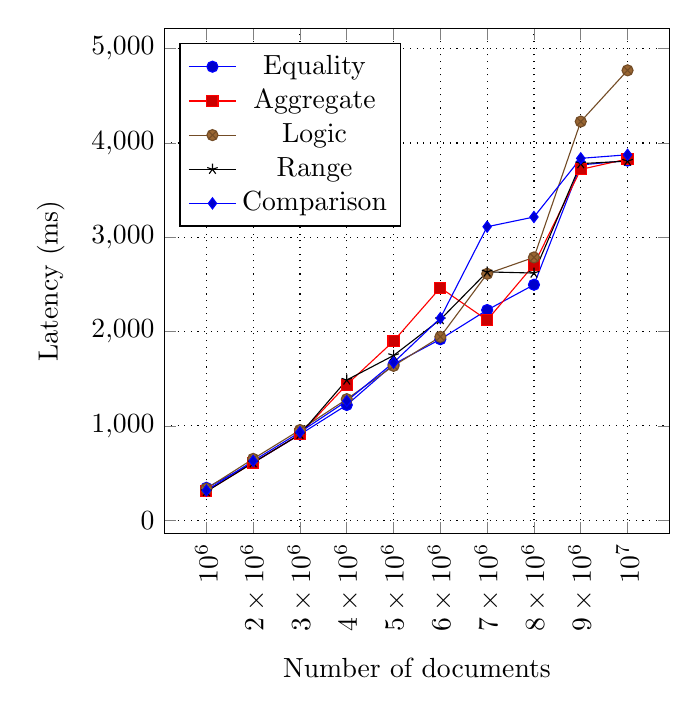
\begin{tikzpicture}
\begin{axis}[legend style={at={(0,0)},anchor=west,at={(axis description cs:1.05,0.45)}},
height=8cm,width=8cm,
ylabel style={yshift=0.1cm},
xlabel style={yshift=-0.1cm},
xlabel={Number of documents},
ylabel={Latency (ms)},
xtick={1,2,3,4,5,6,7,8,9,10},
legend pos=north west,
x tick label style={rotate=90, anchor=east},
xticklabels={$10^6$,$2\times10^6$, $3\times10^6$,$4\times10^6$,$5\times10^6$,$6\times10^6$, $7\times10^6$,$8\times10^6$,$9\times10^6$,$10^7$},
%axis background/.style={fill,bottom color=gray!50,top color=white},
grid=major,
grid style={dotted,black}
]
\addplot+ coordinates {
(1,344)
(2,609)
(3,910)
(4,1222)
(5,1654)
(6,1919)
(7,2229)
(8,2497)
(9,3767)
(10,3813)
};
\addlegendentry{Equality}
\addplot+ coordinates {
(1,306)
(2,610)
(3,911)
(4,1438)
(5,1899)
(6,2465)
(7,2122)
(8,2709)
(9,3720)
(10,3830)
};
\addlegendentry{Aggregate}
\addplot+ coordinates {
(1,335)
(2,651)
(3,957)
(4,1284)
(5,1637)
(6,1945)
(7,2613)
(8,2787)
(9,4227)
(10,4770)
};
\addlegendentry{Logic}
\addplot+ coordinates {
(1,305)
(2,610)
(3,911)
(4,1487)
(5,1747)
(6,2128)
(7,2633)
(8,2621)
(9,3781)
(10,3808)
};
\addlegendentry{Range}
\addplot+ coordinates {
(1,316)
(2,629)
(3,934)
(4,1264)
(5,1672)
(6,2143)
(7,3112)
(8,3215)
(9,3837)
(10,3875)
};
\addlegendentry{Comparison}    
\end{axis}
\end{tikzpicture}
}
\label{fig:LatencyVsSize}
\caption{databases without indexes }
\end{subfigure}
\qquad \qquad
\begin{subfigure}{0.40\textwidth}
\resizebox{0.9\totalheight}{!}{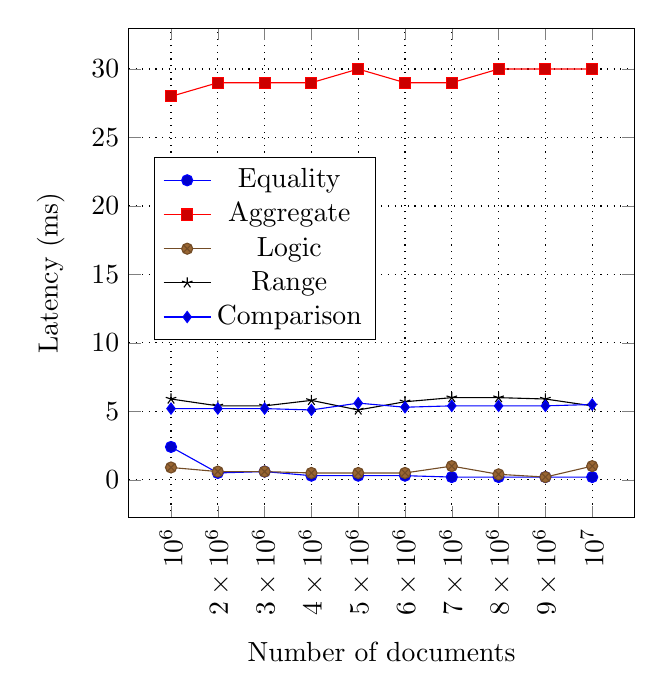
\begin{tikzpicture}
\begin{axis}[legend style={at={(0,0)},anchor=west,at={(axis description cs:.05,0.55)}},
height=7.8cm,width=8cm,
ylabel style={yshift=0.1cm},
xlabel style={yshift=-0.1cm},
xlabel={Number of documents},
ylabel={Latency (ms)},
xtick={1,2,3,4,5,6,7,8,9,10},
%legend pos=north west,
x tick label style={rotate=90, anchor=east},
xticklabels={$10^6$,$2\times10^6$,$3\times10^6$,$4\times10^6$,$5\times10^6$,$6\times10^6$, $7\times10^6$,$8\times10^6$,$9\times10^6$,$10^7$},
%axis background/.style={fill,bottom color=gray!50,top color=white},
grid=major,
grid style={dotted,black}
]
\addplot+ coordinates {
(1,2.4)
(2,0.5)
(3,0.6)
(4,0.3)
(5,0.3)
(6,0.3)
(7,0.2)
(8,0.2)
(9,0.2)
(10,0.2)
};
\addlegendentry{Equality}
\addplot+ coordinates {
(1,28)
(2,29)
(3,29)
(4,29)
(5,30)
(6,29)
(7,29)
(8,30)
(9,30)
(10,30)
};
\addlegendentry{Aggregate}
\addplot+ coordinates {
(1,0.9)
(2,0.6)
(3,0.6)
(4,0.5)
(5,0.5)
(6,0.5)
(7,1)
(8,0.4)
(9,0.2)
(10,1)
};
\addlegendentry{Logic}
\addplot+ coordinates {
(1,5.9)
(2,5.4)
(3,5.4)
(4,5.8)
(5,5.1)
(6,5.7)
(7,6)
(8,6)
(9,5.9)
(10,5.4)
};
\addlegendentry{Range}
\addplot+ coordinates {
(1,5.2)
(2,5.2)
(3,5.2)
(4,5.1)
(5,5.6)
(6,5.3)
(7,5.4)
(8,5.4)
(9,5.4)
(10,5.5)
};
\addlegendentry{Comparison}    
\end{axis}
\end{tikzpicture}}
\label{fig:LatencyWithIndexedDB}
\caption{databases with indexes}
\end{subfigure}
\caption{The performance analysis of query processing as a function of database size. }
\label{queryLatencyToSize}
\end{figure}

%***********************************************************************
\subsection{Results and discussion}
\label{subsec:Discussion}
%***********************************************************************
%The second approach makes true information extraction very difficult, due to formation of fake correlations by insertion of disinformation document. One major draw-back of this method is increase in query processing time as a result of the increasing database size \cite{whang2010managing}.\\ 
%All of the benefits of database technology are transferred to our solution by using standard database server to process encrypted, diluted databases. Indexing is one of these features that significantly improves the query execution time. Detection of correlated attributes in the very large databases demands huge computation power which makes this analysis impractical in most cases. However, S-AQP method with acceptable level of error, can be helpful to calculate the attributes' mutual information, especially, when the chosen sample data is small enough to fit in main memory.

Typical Cloud database services ensure advanced availability and scalability, but the data confidentiality and integrity are yet an area of interest to be explored further. The problem of secure processing of outsourced datasets with limited leakage is investigated in this work. The sensitive data in a single dataset can be protected with using crypto-systems. However, in the cloud DBaaS platform which is a pool of thousands of datasets, the aggregation of datasets introduces a new source of information leakage. The primary goal of this work is that the untrusted DBaaS should learn minimum information from the accumulation of data belonging to the group of users. All risks associated with an untrusted cloud DBaaS is investigated and a mitigation solution is proposed. 

User applications expect to receive valid and accurate information in response of the issued queries, not the fake information. Most NoSQL databases have a different performance with processing the same query over different database size. Our experimental benchmarks demonstrate no significant variations in performance, with a linear increase in the size of database. The small performance penalty is negligible. This can be explained by the multilevel indexing which are utilized by NoSQL databases to provide a fast access time and short latency for query processing over larger databases. To overcome the second challenge, we propose and analyze an efficient algorithm based on the signature schemes to filter out the noisy documents.


%*************************************************
%\subsection{Conclusions and future work}
%\label{subsec:conclusion}
%*************************************************
%For leakage prevention, insertion of disinformation documents is studied to break the links between the documents of among a group of datasets. Simultaneously, insertion of fake documents introduces two types of challenges to the systems. First, along with the data overhead growth, it causes system performance degradation. Second, the increase in communication cost between sever and the proxy which is due to transportation of the fakes documents.   

%We introduced two methods to mitigate the negative effects of data overhead. First, we present leakage quantitative methods to identify the leakage points in datasets; therefore, a selective disinformation document insertion is proposed to minimize leakage just in those points instead of the indiscriminate document insertion. Second, using multi-level indexes. Indexes are one of the most efficient tools to improve query performance by maintaining unique values in a collection. With an index the database process queries by simply scanning the index and fetching documents as they are refereed whereas without index entire table space must be searched. Thus the performance increase is substantial. 
